\documentclass{article}
%Packages
\usepackage{tikz}
\usetikzlibrary{shapes,arrows, positioning}


\begin{document}

\section{How to Draw Rounded Rectangle Shapes}
 
%Method2 (Rounded rectangle shape provide by Tikz library) 

%example1
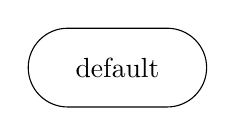
\begin{tikzpicture}
	\node[draw,
	rounded rectangle,
	minimum width=2.5cm,minimum height=1cm]{default}; % whenever you are writing as a rounded rectangle   use rounded rectangle. tit will give you a rounded arc  
\end{tikzpicture}

%example2
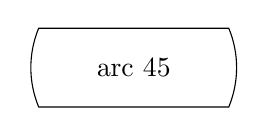
\begin{tikzpicture}
	\node[draw,
	rounded rectangle,
	rounded rectangle arc length=45,
	minimum width=2.5cm,
	minimum height=1cm]{arc 45}; % there is some arc

\end{tikzpicture}

%example3
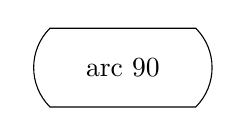
\begin{tikzpicture}
	\node[draw,
	rounded rectangle,
	rounded rectangle arc length=90,
	minimum width=2.5cm,
	minimum height=1cm]{arc 90};
\end{tikzpicture}


%Method1 (standard rectangle with rounded corners option

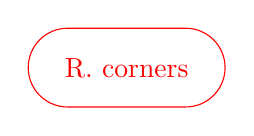
\begin{tikzpicture}
	\node[draw,
	rounded corners=0.5cm,
	minimum width=2.5cm,
	minimum height=1cm,red]{R. corners}; %text also red, color also red.

\end{tikzpicture}


\end{document}


